This section describes the schema currently used to store
\glspl{fragilitymodel}, which are required for the Scenario Damage Calculator
and the Classical Probabilistic Seismic Damage Calculator. In order to perform
probabilistic or scenario damage calculations, it is necessary to define a
\gls{fragilityfunction} for each building typology present in the
\gls{exposuremodel}. A \gls{fragilitymodel} defines a set of
\glspl{fragilityfunction}, describing the probability of exceeding a set of
limit, or damage, states. The \glspl{fragilityfunction} can be defined using
either a discrete or a continuous format, and the \gls{fragilitymodel} file
can include a mix of both types of \glspl{fragilityfunction}.

For discrete \glspl{fragilityfunction}, sets of probabilities of exceedance
(one set per limit state) are defined for a list of intensity measure levels,
as illustrated in Figure~\ref{fig:fragility-discrete}.

\begin{figure}[ht]
\centering
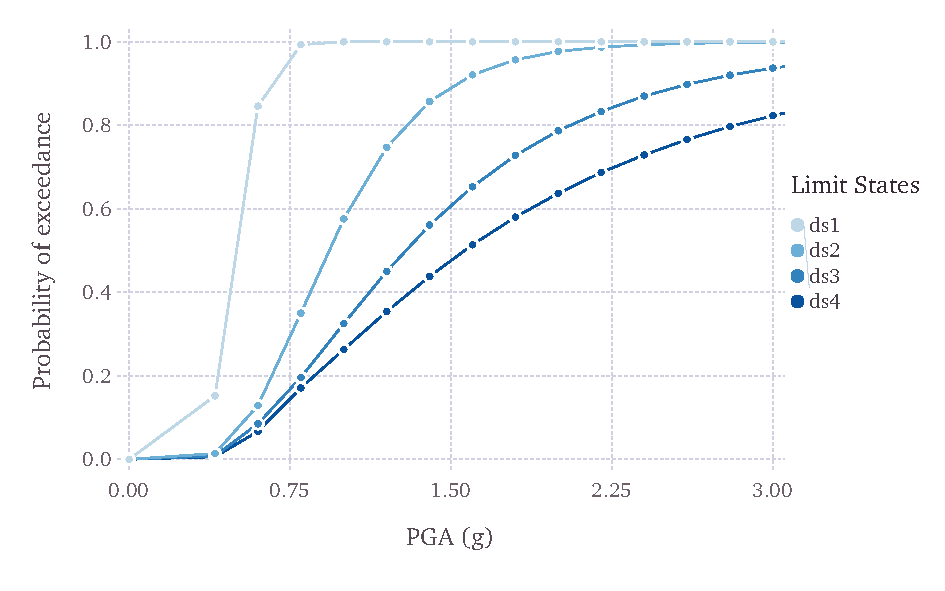
\includegraphics[width=12cm]{figures/risk/fragility-discrete.pdf}
\caption{Graphical representation of a discrete fragility model}
\label{fig:fragility-discrete}
\end{figure}

The \glspl{fragilityfunction} can also be defined as continuous functions,
through the use of cumulative lognormal distribution functions. In
Figure~\ref{fig:fragility-continuous}, a continuous \gls{fragilitymodel} is
presented.

\begin{figure}[ht]
\centering
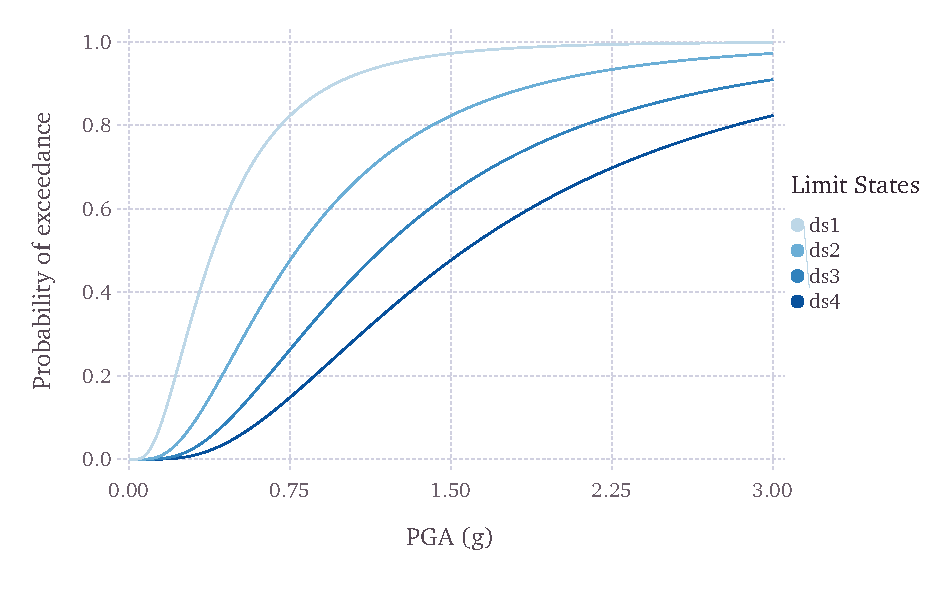
\includegraphics[width=12cm]{figures/risk/fragility-continuous.pdf}
\caption{Graphical representation of a continuous fragility model}
\label{fig:fragility-continuous}
\end{figure}

An example \gls{fragilitymodel} comprising one discrete
\gls{fragilityfunction} and one continuous \gls{fragilityfunction} is shown in
Listing~\ref{lst:input_fragility}.

\begin{listing}[htbp]
  \inputminted[firstline=1,firstnumber=1,fontsize=\footnotesize,frame=single,linenos,bgcolor=lightgray]{xml}{oqum/risk/Verbatim/input_fragility.xml}
  \caption{Example fragility model comprising one discrete fragility function and one continuous fragility function (\href{https://raw.githubusercontent.com/GEMScienceTools/oq-engine-docs/master/oqum/risk/verbatim/input_fragility.xml}{Download example})}
  \label{lst:input_fragility}
\end{listing}


The initial portion of the schema contains general information that describes
some general aspects of the \gls{fragilitymodel}. The information in this
metadata section is common to all of the functions in the \gls{fragilitymodel}
and needs to be included at the beginning of every \gls{fragilitymodel} file.
The parameters of the metadata section are shown in the snippet below and
described after the snippet:

\inputminted[firstline=4,firstnumber=4,lastline=9,fontsize=\footnotesize,frame=single,linenos,bgcolor=lightgray]{xml}{oqum/risk/Verbatim/input_fragility.xml}

\begin{itemize}

    \item \Verb+id+: mandatory; a unique string used to identify the 
      \gls{fragilitymodel}. This string can contain letters~(a--z; A--Z), 
      numbers~(0--9), dashes~(-), and underscores~(\_), with a maximum of 
      100~characters.

    \item \Verb+assetCategory+: an optional string used to specify the type of
      \glspl{asset} for which \glspl{fragilityfunction} will be defined in this
      file (e.g: buildings, lifelines).

    \item \Verb+lossCategory+: mandatory; valid strings for this attribute are 
      ``structural'', ``nonstructural'', ``contents'', and 
      ``business\_interruption''.

    \item \Verb+description+: mandatory; a brief string (ASCII) with further 
      relevant information about the \gls{fragilitymodel}, 
      for example, which building typologies are covered
      or the source of the functions in the \gls{fragilitymodel}.

    \item \Verb+limitStates+: mandatory; this field is used to define the number and 
      nomenclature of each limit state. Four limit states are employed in the 
      example above, but it is possible to use any number of discrete states,
      as long as a fragility curve is always defined for each limit state. The 
      limit states must be provided as a set of strings separated by whitespaces 
      between each limit state. Each limit state string can contain
      letters~(a--z; A--Z), numbers~(0--9), dashes~(-), and underscores~(\_).
      Please ensure that there is no whitespace within the name of any
      individual limit state.

\end{itemize}



The following snippet from the above \gls{fragilitymodel} example file defines a
discrete \gls{fragilityfunction}:

\inputminted[firstline=11,firstnumber=11,lastline=17,fontsize=\footnotesize,frame=single,linenos,bgcolor=lightgray]{xml}{oqum/risk/Verbatim/input_fragility.xml}

The following attributes are needed to define a discrete \gls{fragilityfunction}:

\begin{itemize}

    \item \Verb+id+: mandatory; a unique string used to identify the 
      \gls{taxonomy} for which the function is being defined. This string is
      used to relate the \gls{fragilityfunction} with the relevant \gls{asset}
      in the \gls{exposuremodel}. This string can contain letters~(a--z; A--Z),
      numbers~(0--9), dashes~(-), and underscores~(\_), with a maximum of
      100~characters.

    \item \Verb+format+: mandatory; for discrete \glspl{fragilityfunction}, this
      attribute should be set to ``\Verb+discrete+''.

    \item \Verb+imls+: mandatory; this attribute specifies the list of intensity levels
      for which the limit state probabilities of exceedance will be defined. 
      In addition, it is also necessary to define the intensity measure type 
      (\Verb+imt+). Optionally, a \Verb+noDamageLimit+ can be specified, which 
      defines the intensity level below which the probability of exceedance 
      for all limit states is taken to be zero.

    \item \Verb+poes+: mandatory; this field is used to define the probabilities of 
      exceedance (\Verb+poes+) for each limit state for each discrete 
      \gls{fragilityfunction}. It is also necessary to specify which limit 
      state the exceedance probabilities are being defined for using the 
      attribute \Verb+ls+. The probabilities of exceedance for each limit state
      must be provided on a separate line; and the number of exceedance 
      probabilities for each limit state defined by the \Verb+poes+ attribute 
      must be equal to the number of intensity levels defined by the attribute 
      \Verb+imls+. Finally, the number and names of the limit states in each 
      fragility function must be equal to the number of limit states defined 
      earlier in the metadata section of the \gls{fragilitymodel} using the 
      attribute \Verb+limitStates+.

\end{itemize}



The following snippet from the above \gls{fragilitymodel} example file
defines a continuous \gls{fragilityfunction}:

\inputminted[firstline=19,firstnumber=19,lastline=25,fontsize=\footnotesize,frame=single,linenos,bgcolor=lightgray]{xml}{oqum/risk/Verbatim/input_fragility.xml}

The following attributes are needed to define a continuous \gls{fragilityfunction}:

\begin{itemize}

    \item \Verb+id+: mandatory; a unique string used to identify the 
      \gls{taxonomy} for which the function is being defined. This string is
      used to relate the \gls{fragilityfunction} with the relevant \gls{asset}
      in the \gls{exposuremodel}. This string can contain letters~(a--z; A--Z),
      numbers~(0--9), dashes~(-), and underscores~(\_), with a maximum of
      100~characters.

    \item \Verb+format+: mandatory; for continuous \glspl{fragilityfunction},
      this attribute should be set to ``\Verb+continuous+''.

    \item \Verb+shape+: mandatory; for continuous \glspl{fragilityfunction}
      using the lognormal cumulative distrution, this attribute should be set
      to ``\Verb+logncdf+''. At present, only the lognormal cumulative
      distribution function can be used for representing continuous
      \glspl{fragilityfunction}.

    \item \Verb+imls+: mandatory; this element specifies aspects related to the
      intensity measure used by the the \gls{fragilityfunction}. The range of 
      intensity levels for which the continuous \glspl{fragilityfunction} are valid
      is specified using the attributes \Verb+minIML+ and \Verb+maxIML+. 
      In addition, it is also necessary to define the intensity measure type 
      \Verb+imt+. Optionally, a \Verb+noDamageLimit+ can be specified, which 
      defines the intensity level below which the probability of exceedance 
      for all limit states is taken to be zero.

    \item \Verb+params+: mandatory; this field is used to define the parameters
      of the continuous curve for each limit state for this 
      \gls{fragilityfunction}. For a lognormal cumulative distrbution function, 
      the two parameters required to specify the function are the mean and 
      standard deviation of the intensity level. These parameters are defined for 
      each limit state using the attributes \Verb+mean+ and \Verb+stddev+ 
      respectively. The attribute \Verb+ls+ specifies the limit state for which 
      the parameters are being defined. The parameters for each limit state
      must be provided on a separate line. The number and names of the limit 
      states in each \gls{fragilityfunction} must be equal to the number of limit 
      states defined earlier in the metadata section of the \gls{fragilitymodel}
      using the attribute \Verb+limitStates+.

\end{itemize}


Note that the schema for representing \glspl{fragilitymodel} has changed
between \gls{acr:nrml} v0.4 (used prior to \gls{acr:oqe17}) and \gls{acr:nrml}
v0.5 (introduced in \gls{acr:oqe17}).

A deprecation warning is printed every time you attempt to use a
\gls{fragilitymodel} in the old \gls{acr:nrml} v0.4 format in an
\gls{acr:oqe17} (or later) risk calculation. To get rid of the warning you
must upgrade the old \glspl{fragilitymodel} files to \gls{acr:nrml} v0.5. You
can use the command \Verb+upgrade_nrml+ with oq to do this as follows:

\begin{minted}[fontsize=\footnotesize,frame=single,bgcolor=lightgray]{shell-session}
user@ubuntu:~\$ oq upgrade_nrml <directory-name>
\end{minted}

The above command will upgrade all of your old \gls{fragilitymodel} files to
\gls{acr:nrml} v0.5. The original files will be kept, but with a .bak extension
appended. Notice that you will need to set the \Verb+lossCategory+ attribute
to its correct value manually. This is easy to do, since if you try to run a
computation you will get a clear error message telling the expected value for
the \Verb+lossCategory+ for each file.


Several methodologies to derive \glspl{fragilityfunction} are currently being
evaluated by \gls{acr:gem} and have been included as part of the Risk
Modeller's Toolkit, the code for which can be found on a public repository at
GitHub at the following address: 
\href{http://github.com/gemsciencetools/rmtk}{http://github.com/gemsciencetools/rmtk}.

A web-based tool to build a \gls{fragilitymodel} in the \gls{acr:nrml} schema
are also under development, and can be found at the OpenQuake platform at the
following address: \href{https://platform.openquake.org/ipt/}{https://platform.openquake.org/ipt/}.